\documentclass[a4paper]{article}
\usepackage{graphicx}

\begin{document}

	\title{\Huge{Software Requirement Specification}}
	\author{Group 8}
	\maketitle

	\section{Introduction}

		Introduction

	\section{Vision}

		Vision

	\section{Background}

		Background

	\section{Architectural Requirements}

		\subsection{Access Channel Requiremnets}

			\begin{itemize}

				\item{An Item}

				\item{Another Item}

			\end{itemize}

		\subsection{Quality Requirements}

			\begin{enumerate}

				\item{An Item}

				\item{Another Item}

			\end{enumerate}

		\subsection{Integration Requirements}

			\begin{description}

				\item[first]{An Item}

				\item[second]{Another Item}

			\end{description}

		\subsection{Architecture Constraints}

	\section{Functional Requirements}

		\subsection{Introduction}

			This section is an introduction into the functional requirements of the system.

		\subsection{Scope and Limitations/Exclusions}
		
			\begin{figure}[h]
				\caption{High Level Use Case Diagram}
				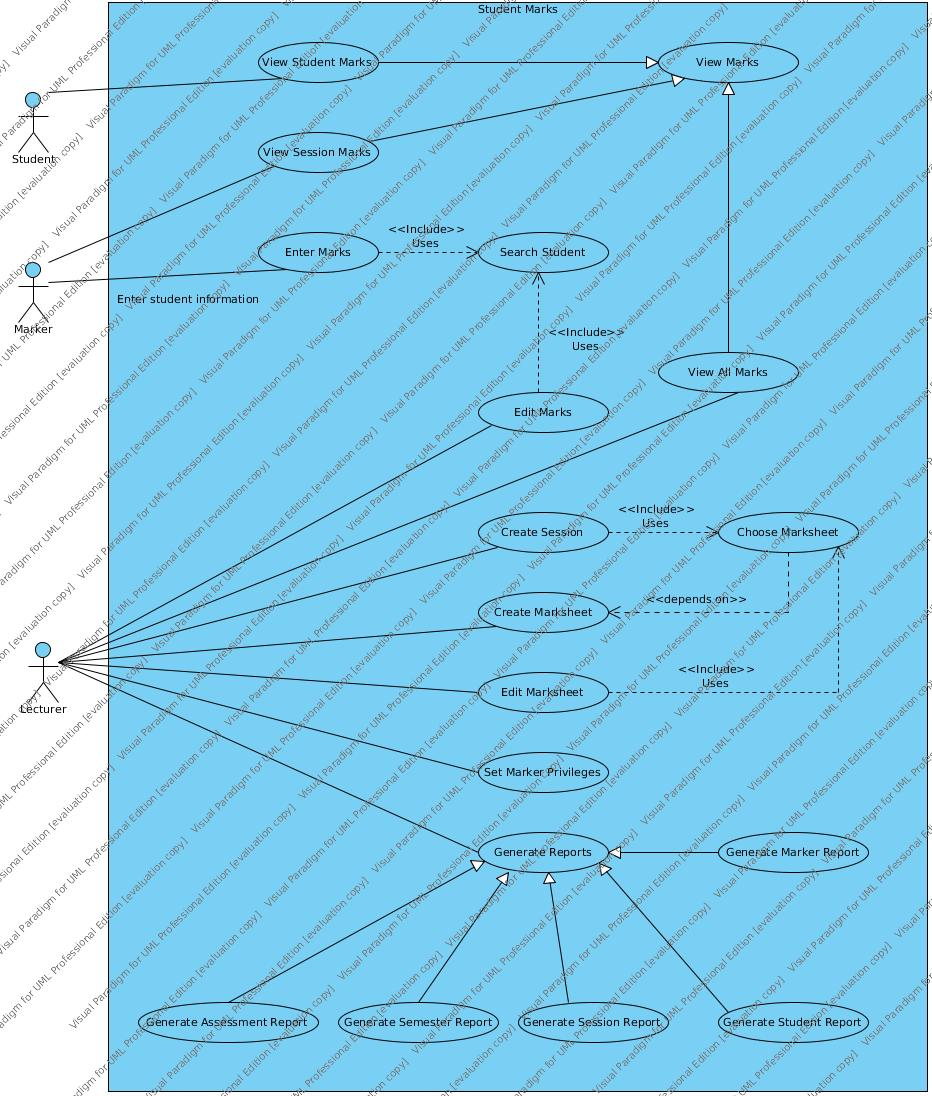
\includegraphics[height=15cm]{StudentMarks}
			\end{figure}

		\subsection{Required Functionality}

		\subsection{Use Case Prioritisation}

		\subsection{Use Case/Service Contracts}

		\subsection{Process Specification}

		\subsection{Domain Objects}

	\section{Open Issues}

	\section{Glossary}

\end{document}